\documentclass[conference]{IEEEtran}
\IEEEoverridecommandlockouts
% The preceding line is only needed to identify funding in the first footnote. If that is unneeded, please comment it out.
\usepackage{cite}
\usepackage{amssymb,amsfonts, mathtools}
\usepackage{amsmath}
\usepackage{bm}
\interdisplaylinepenalty=2500
\DeclareMathOperator{\sgn}{sgn}
\DeclarePairedDelimiter{\ceil}{\lceil}{\rceil}
\DeclarePairedDelimiter{\floor}{\lfloor}{\rfloor}
\usepackage{algorithmic}
\usepackage[serbian]{babel}
\usepackage{graphicx}
\usepackage{textcomp}
\usepackage{hyperref}
\usepackage{xcolor}
\def\BibTeX{{\rm B\kern-.05em{\sc i\kern-.025em b}\kern-.08em
		T\kern-.1667em\lower.7ex\hbox{E}\kern-.125emX}}

% --------------------------------------------------------------------------------------
\begin{document}

\title{Sistem za direktnu digitalnu sintezu}

\author{\IEEEauthorblockN{Kristijan Mitrović}
\IEEEauthorblockA{\textit{Odsek za elektroniku} \\
	\textit{Elektrotehnički fakultet}\\
	Beograd, Srbija \\
	mk150214d@student.etf.bg.ac.rs}
\and
\IEEEauthorblockN{ Dragan Božinović}
\IEEEauthorblockA{\textit{Odsek za elektroniku} \\
	\textit{Elektrotehnički fakultet}\\
	Beograd, Srbija \\
	bd150211d@student.etf.bg.ac.rs}
}

\maketitle

% -------------------------- Abstract ------------------------------------------------
\begin{abstract}
Ovaj rad predstavlja rešenje projekta iz predmeta \textsl{Hardversko-softverska obrada signala}. U odeljku \ref{sekcija:problem} opisan je sistem za direktnu digitalnu sintezu koji je potrebno realizovati. U odeljku \ref{sekcija:teorija} izvršena je detaljna teorijska analiza navedenog sistema i dat predlog za implementaciju. Razvojno okruženje u okviru kojeg je izvršena implementacija, kao i sama implementacija, dati su u odeljcima \ref{sekcija:okruzenje} i \ref{sekcija:kod}, respektivno.
\end{abstract}

% ------------------------- Problem ---------------------------------------------------
\section{Postavka problema}\label{sekcija:problem}
Potrebno je realizovati sistem za direktnu digitalnu sintezu (DDS), prikazan na slici \ref{slika:dds}, koji se koristi za generisanje sinusnog signala u opsegu učestanosti $[\Delta f, f_{max}]$.

\begin{figure}[h]
	\centering
	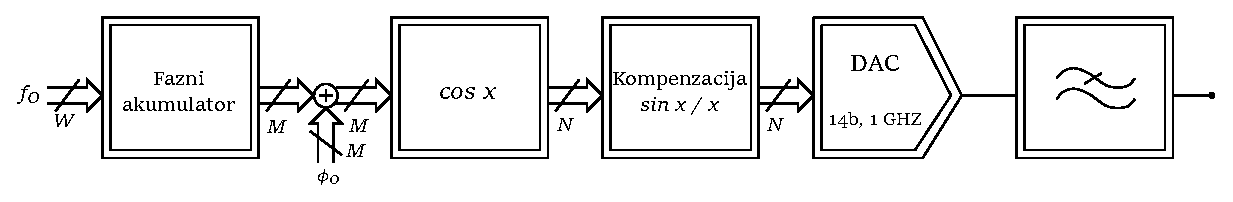
\includegraphics[scale=0.43]{./slike/dds.eps}
	\caption{\textsl{Blok dijagram DDS sistema}}
	\label{slika:dds}
\end{figure}

Učestanost generisanog signala se zadaje $W$-bitnom kontrolnom rečju $f_0$, dok se početna faza može zadati kontrolnom rečju $\phi_0$. Pretpostavka je da se ceo sistem taktuje signalom učestanosti $f_{clk} = 100$\,MHz i da je $f_{max} = 40$\,MHz. \\

Potrebno je:
\begin{itemize}
	\item Odrediti širinu $W$ kontrolne reči $f_0$ tako da frekvencijska rezolucija DDS sistema bude $\Delta f = 100\,\mu$Hz.
	\item Predložiti arhitekturu generatora odbiraka $cos\,x$ i moguće optimizacije. Proceniti složenost implementacije.
	\item Odrediti red i koeficijente FIR filtra za korekciju $sin\,x/x$ frekvencijske karakteristike kola zadrške nultog reda, tako da varijacija amplitude izlaznog signala bude $\pm 0.05$\,dB u opsegu učestanosti od interesa.
	\item Odrediti specifikacije analognog rekonstrukcionog filtra tako da spektralne replike budu potisnute bar $60$\,dB. Na osnovu specifikacija predložiti tip i red analognog filtra.
	\item Predložiti arhitekturu faznog modulatora i/ili modifikaciju arhitekture DDS-a za potiskivanje spurova usled kvantizacije faze i amplitude.
	\item Izračunati maksimalni džiter signala takta $t_{j,clk}$ za koji ne dolazi do degradacije signala maksimalne učestanosti u prvoj i višim Nikvistovim zonama. Predložiti adekvatan izvor signala takta i izracunati džiter na osnovu profila faznog šuma.
	\item Razmotriti potrebne modifikacije i ograničenja za generisanje signala u trećoj Nikvistovoj zoni. Proračunati parametre modifikovanih blokova.
\end{itemize}
\bigskip

% ------------------------- Teorijsko resenje --------------------------------------
\section{Teorijsko rešenje}\label{sekcija:teorija}
% ------------------------- W ---------------------------------------------------
\subsection{Fazni akumulator}
Fazni akumulator je deo sistema koji se taktuje sa $f_{clk}$ i koji na svaki takt uvećava svoj sadržaj za bezdimenzionu vrednost $\Delta \theta$. Neka je, primera radi, $W=4$ i $\Delta \theta=0001_b$, a početna vrednost u faznom akumulatoru $0000_b$. Na svaki takt vrednost u faznom akumulatoru se inkrementira za $0001$, odakle je posle jednog takta u njemu zapisano $0001_b$, posle drugog $0010_b$ itd., sve dok nakon $2^4=16$ taktova ne dođe do prekoračenja $1111_b\rightarrow 0000_b$, nakon čega se ciklus ponavlja. Ovakvo ponašanje, nastalo kao posledica ograničene aritmetike, omogućava mapiranje vrednosti faznog akumulatora u ugao jediničnog vektora koji rotira u faznoj ravni, kao što je prikazano na slici \ref{slika:faznaravan}. 

\begin{figure}[h]
	\centering
	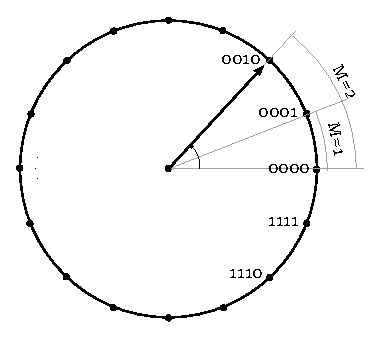
\includegraphics[scale=0.6]{./slike/faznaravan.eps}
	\caption{\textsl{Rotacija vektora u faznoj ravni}}
	\label{slika:faznaravan}
\end{figure}

Krug je podeljen na $2^W$ delova, gde razmak između dve sukcesivne tačke na kružnici predstavlja najmanji mogući inkrement faze koji je jednak $40$-obitnom broju kod koga su svi biti sem najnižeg nule. Dakle, najmanji inkrement faze je $\Delta \theta_{min}=00\ldots01_b$. Pri obilasku kružnice za inkrement faze koji nije najmanji, događa se da se neke tačke preskaču, čime se efektivno postiže da se krug obiđe više puta za isto vreme, tj.~veća frekvencija sinusa čiji je argument ova faza. Na osnovu toga može se napisati

\begin{equation}
f_{0} = M_{inc}\,\frac{f_{clk}}{2^W} ,
\end{equation}

\noindent gde je $M_{inc}$ faktor koji diktira ''preskakanje`` tačaka na kružnici, a $f_{0}$ učestanost izlaznog sinusa. Odavde se može izraziti najmanji inkrement frekvencije kao

\begin{equation}\label{eq:deltaf}
\Delta f = \frac{f_{clk}}{2^W} ,
\end{equation}

\noindent i faktor inkrementa kao

\begin{equation}\label{eq:Minc}
M_{inc} = \frac{f_{0}}{f_{clk}}\,2^W .
\end{equation}

Iz (\ref{eq:deltaf}) se preuređivanjem dobija da je 

\begin{equation}
W = \ceil[\Big]{\log_2{\frac{f_{clk}}{\Delta f}}} ,
\end{equation}

\noindent što daje $W = 40$ za zadate brojne vrednosti. 
Jednačina (\ref{eq:Minc}) omogućava da se za unetu željenu učestanost izlaznog sinusa dobije inkrement $\Delta \theta=M_{inc}\,\Delta \theta_{min}$ kojim se sadržaj faznog akumulatora uvećava na svaki takt. 

S obzirom da je \textsl{DAC} $14$-obitni, $N$ je fiksirano na $14$. Kao maksimalna smislena vrednost za $M$ takođe se nameće $14$, budući da je time obezbeđeno jednoznačno mapiranje ulaza u generator odbiraka u vrednosti njegovih izlaza.

Najviših $14$ bita faznog akumulatora iskorišćeno je za mapiranje faze u $[0, 2\pi]$. Od tih $14$ bita, $12$ nižih bita iskorišćeno je za mapiranje ugla $[0, \pi/2]$ u $[0, 2^{12}]$, dok su preostala dva iskorišćena kao indikator kvadranta u kom se ugao nalazi. Na slici \ref{slika:fazniAcc} plavom bojom prikazana je vrednost unutar faznog akumulatora, a crvenom njegov $12$-obitni izlaz za jednu punu rotaciju u faznoj ravni pri $M_{inc}=1$. Crveni signal se direktno vodi na generator odbiraka.

\begin{figure}[h]
	\centering
	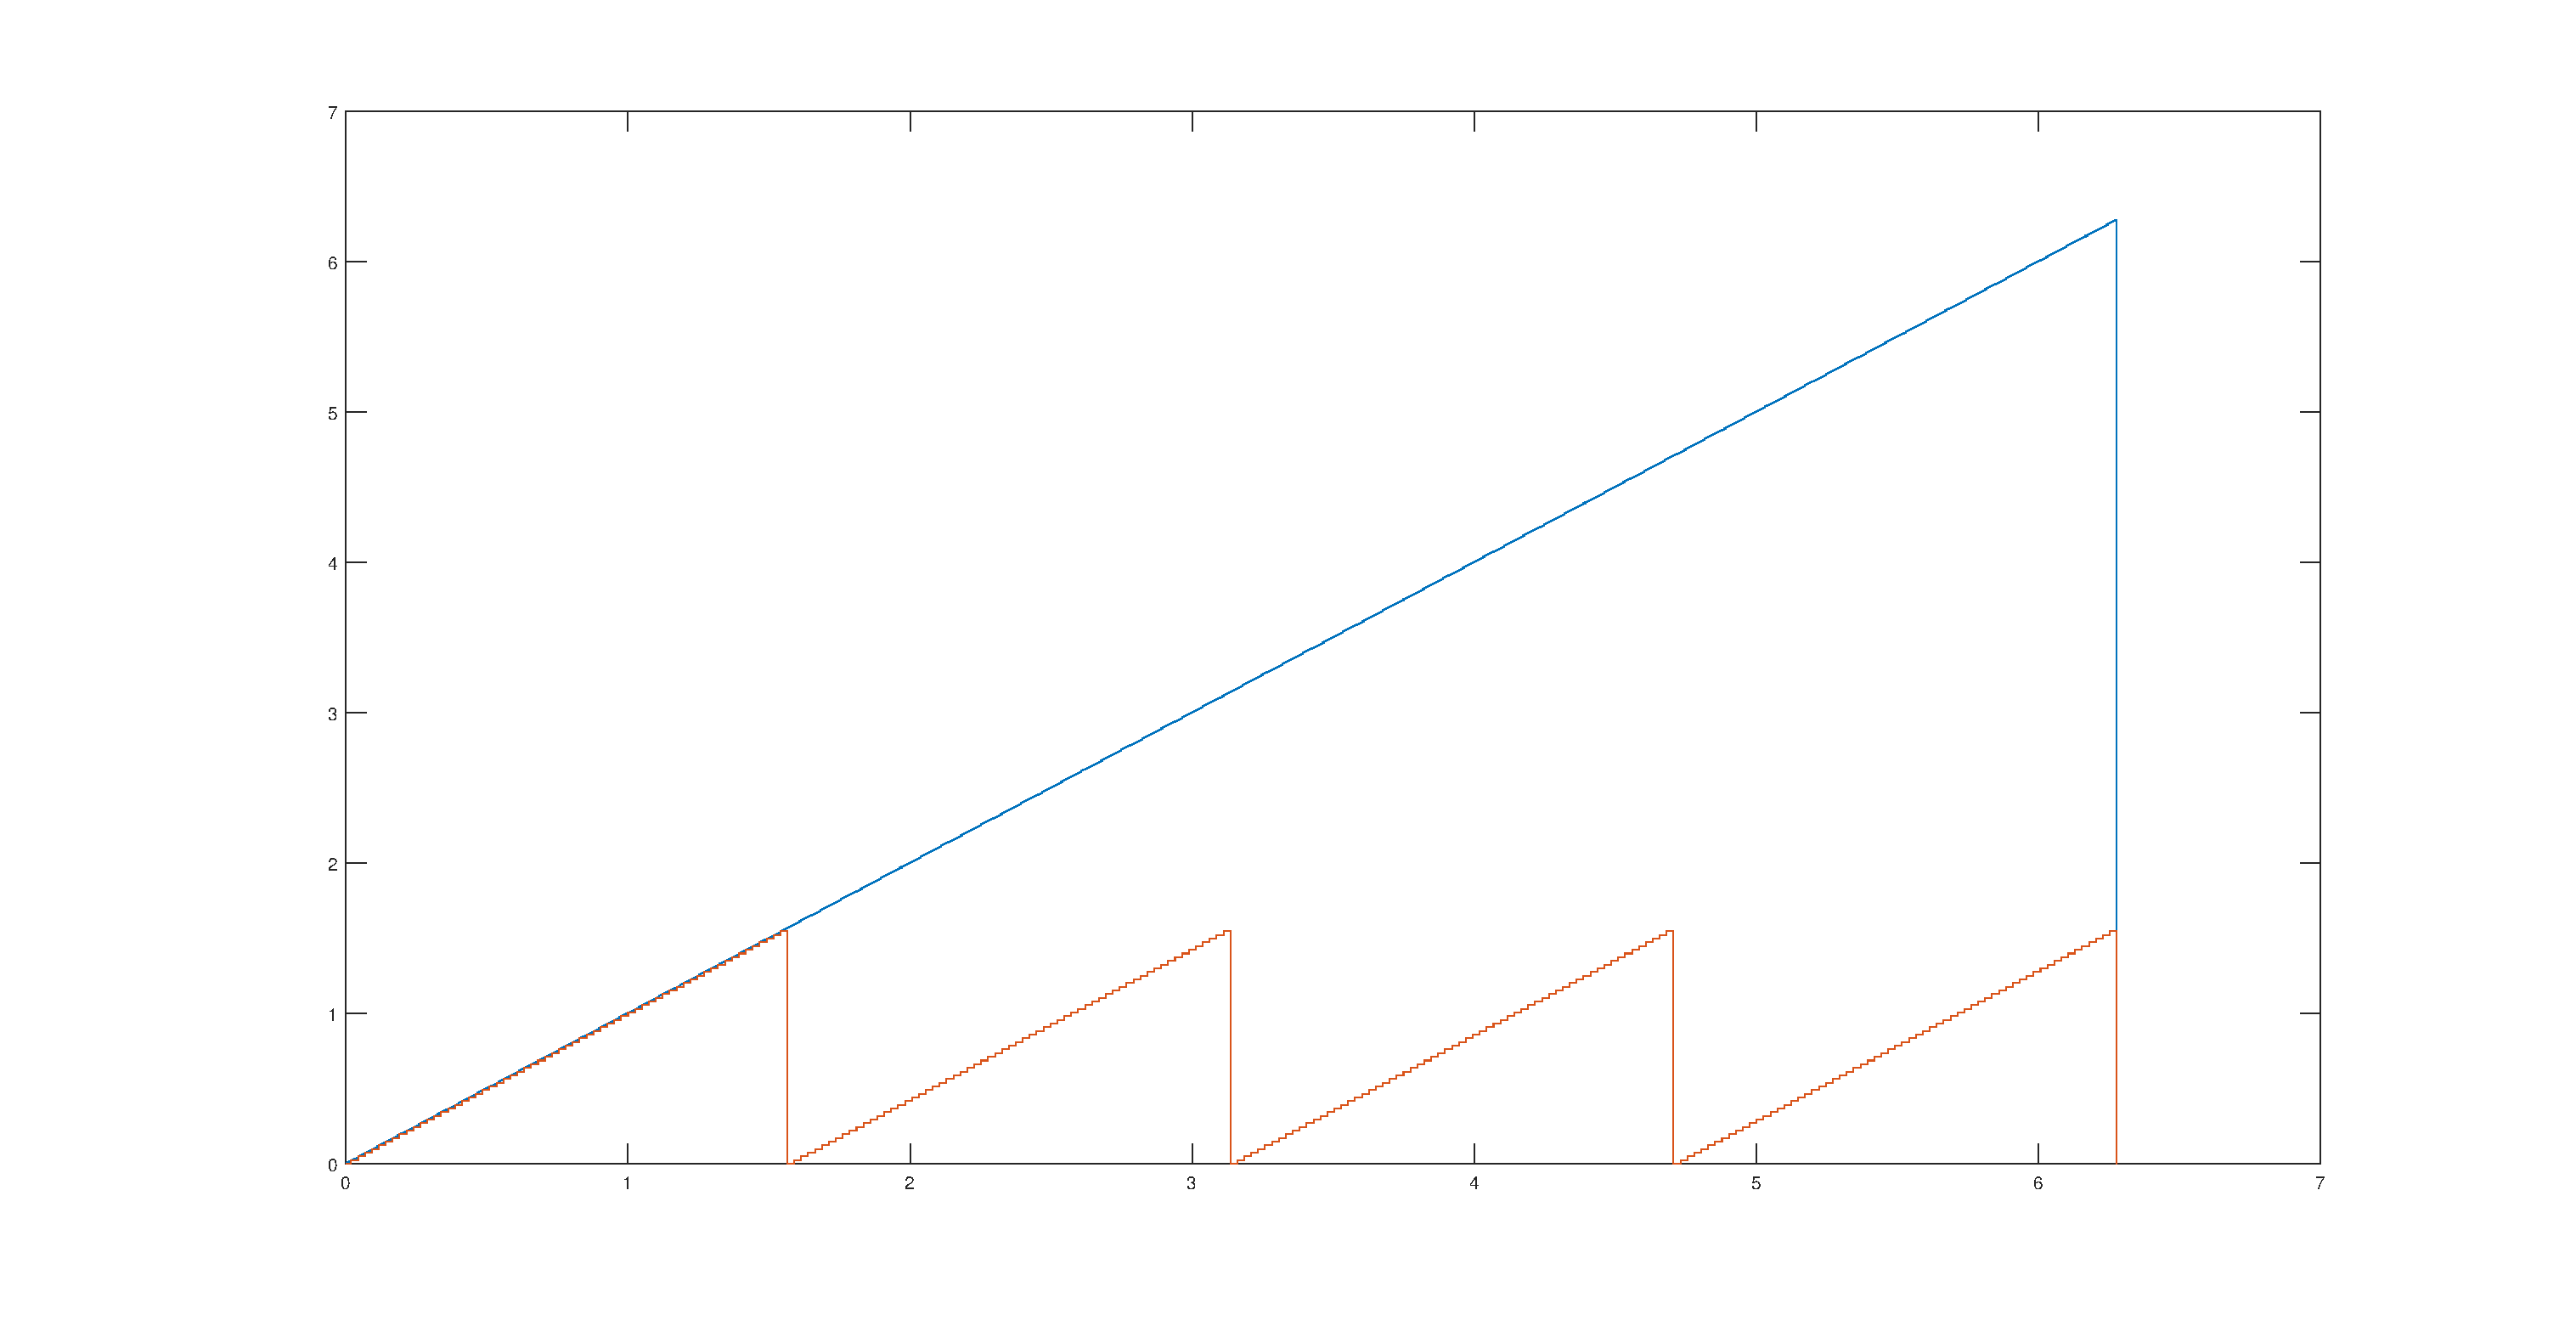
\includegraphics[scale=0.16]{./slike/izlazFaznogAkumulatora.eps}
	\caption{\textsl{Izlaz faznog akumulatora}}
	\label{slika:fazniAcc}
\end{figure}

% ------------------ cos x -------------------------------------------
\subsection{Generator odbiraka $cos\,x$}
Jedna mogućnost za generisanje amplitude na osnovu argumenta kosinusne funkcije je \textsl{look-up} tabela. Prednost ovog pristupa je što se vrednost amplitude ne proračunava u toku izvršavanja, već se prostim indeksiranjem tabele (niza) iz nje dovhata prethodno izračunata vrednost, što se može obaviti vrlo brzo. Ukoliko nikakve metode kompresije nisu primenjene (recimo, čuvanje amplituda samo za četvrtinu uglova, imajući u vidu simetriju sinusnog signala, ili neke optimizacije sa bitima), tabela će imati $2^M=2^{14}$ ulaza, što je $14\times 2^{14}=28$\,kB podataka smeštenih u \textsl{ROM} memoriju. Imajući u vidu da je, recimo, veličina \textsl{EEPROM} memorije kod \textsl{Arudino Uno} mikrokontrolera $1$\,kB, postaje jasno zašto ovakav pristup nije praktičan. Povećanjem broja bita sa $n$ na $n+1$, broj ulaza u tabelu se duplira, što znači eksponencijalnu složenost u zahtevima za memorijom. 

Sa druge strane, \textsl{CORDIC} algoritam se vrlo često primenjuje kod generisanja elementarnih, hiperboličkih i trigonometrijskih funkcija, kao i kod numerički kontrolisanih oscilatora, što je situacija sa \textsl{DDS} sistemom koji ovde razmatramo. Čisto softverska implementacija \textsl{CORDIC}-a zahteva proste iteracije kroz petlju u kojoj se vrše operacije sabiranja, oduzimanja i pomeranja, a maksimalna greška aproksimacije ugla, kao i povećanje rezolucije za jedan bit, mogu se obezbediti povećanjem broja iteracija.

Za izračunavanje sinusa i kosinusa ugla, \textsl{CORDIC} algoritam se primenjuje u tzv.~\textit{rotacionom} modu. Algoritam se sastoji iz $M$ iteracija kroz petlju u kojoj se vrše sledeća izračunavanja:

\begin{align}
x_{i+1} &= x_i - \sigma_i y_i \gg i , \label{eq:cordicX}		\\
y_{i+1} &= y_i + \sigma_i x_i \gg i  ,		\\
z_{i+1} &= z_i - \sigma_i\arctan{2^{-i}} ,		\\
\sigma_i &= \sgn(z_i) \label{eq:cordicSigma} .
\end{align}

Rotacija vektora za ugao $\theta$ može se izvršiti u više koraka, odnosno mikrorotacija:

\begin{equation}
\bm{ROT}(\theta) = \prod_i{\bm{ROT}(\sigma_i\,\theta_i)}
\end{equation}

Imajući u vidu da je

\begin{equation}
	\begin{split}
		\bm{ROT}(\sigma_i\,\theta_i) & = 
		\begin{bmatrix}
			\cos \sigma_i\,\theta_i & -\sin \sigma_i\,\theta_i \\
			\sin \sigma_i\,\theta_i & \cos \sigma_i\,\theta_i \\
		\end{bmatrix} ,
	\end{split}
\end{equation}

\noindent i pogodnim odabirom $\theta_i = \arctan 2^{-i}$, dobija se da je 

\begin{equation}
	\begin{split}
		\bm{ROT}(\sigma_i\,\theta_i) & = 
		\frac{1}{\sqrt{1+2^{-2i}}}\,
		\begin{bmatrix}
			1 & -\sigma_i\,2^{-i} 	\\
			\sigma_i\,2^{-i}	&	1 \\
		\end{bmatrix} .
	\end{split}
\end{equation}

Izraz koji množi matricu je multiplikativni faktor $K(i)$, koji se za zadati broj mikrorotacija $n$ može unapred izračunati kao

\begin{equation}\label{eq:Kinf}
K(n) = \prod_{i=0}^{n-1}{K_i} = \prod_{i=0}^{n-1}{\frac{1}{\sqrt{1+2^{-2i}}}},
\end{equation}

\noindent čija granična vrednost za $n\rightarrow \infty$ iznosi $K_{\infty}\approx 0.60726$. 

Kako se generatoru signala, na osnovu blok dijagrama sa slike \ref{slika:dds}, dostavlja vrednost argumenta na osnovu koje treba da generiše amplitudu, mora se u obzir uzeti i vreme potrebno za izračunavanje izraza (\ref{eq:cordicX}) -- (\ref{eq:cordicSigma}). Od $W$ bita, generatoru odbiraka dovodi se $M$ najviših bita faznog akumulatora, čime je obezbeđeno $2^{W-M}$ taktova vremena da algoritam sračuna amplitudu za vrednost argumenta koja je trenutno na njegovom ulazu, pre nego fazni akumulator promeni taj argument.

Na slici \ref{slika:sin} prikazan je izlaz generatora odbiraka kada se na njegov ulaz dovede crveni signal sa slike \ref{slika:fazniAcc}. Prostim povećanjem $M_{inc}$ sa $1$ na $2$ dobija se sinus duplo veće učestanosti sa slike \ref{slika:sin2}.

\begin{figure}[h!]
	\centering
	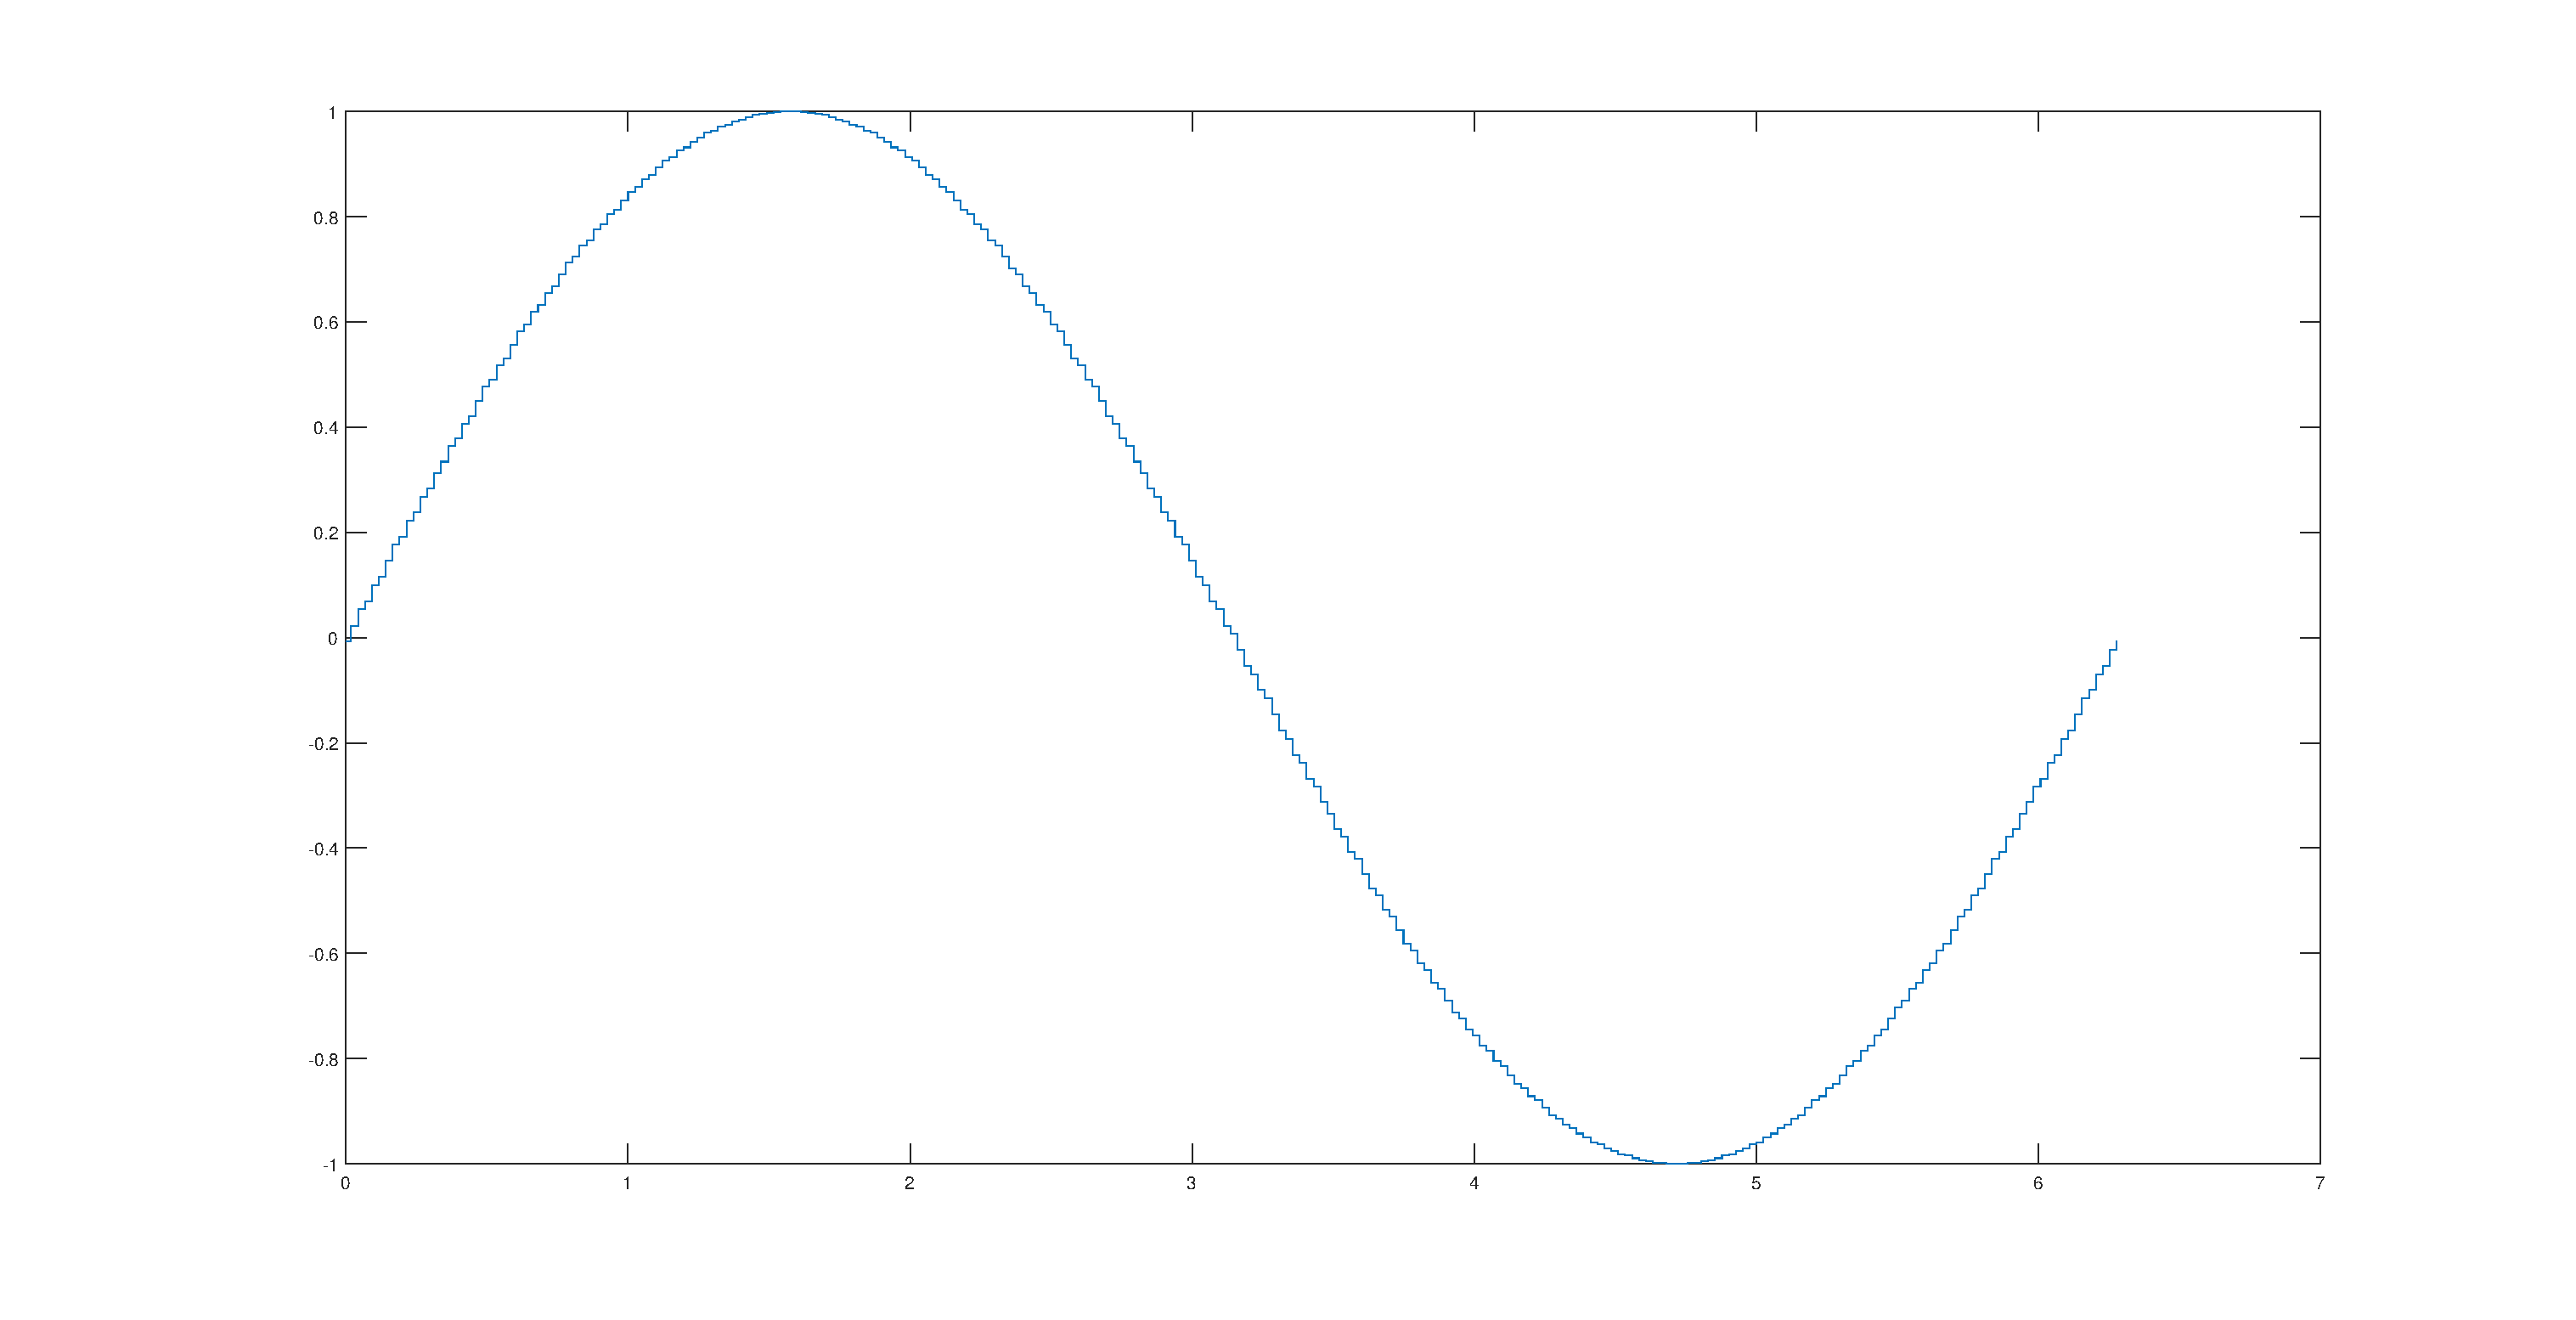
\includegraphics[scale=0.16]{./slike/sinus.eps}
	\caption{\textsl{Sinus osnovne učestanosti}}
	\label{slika:sin}
\end{figure}

\begin{figure}[h!]
	\centering
	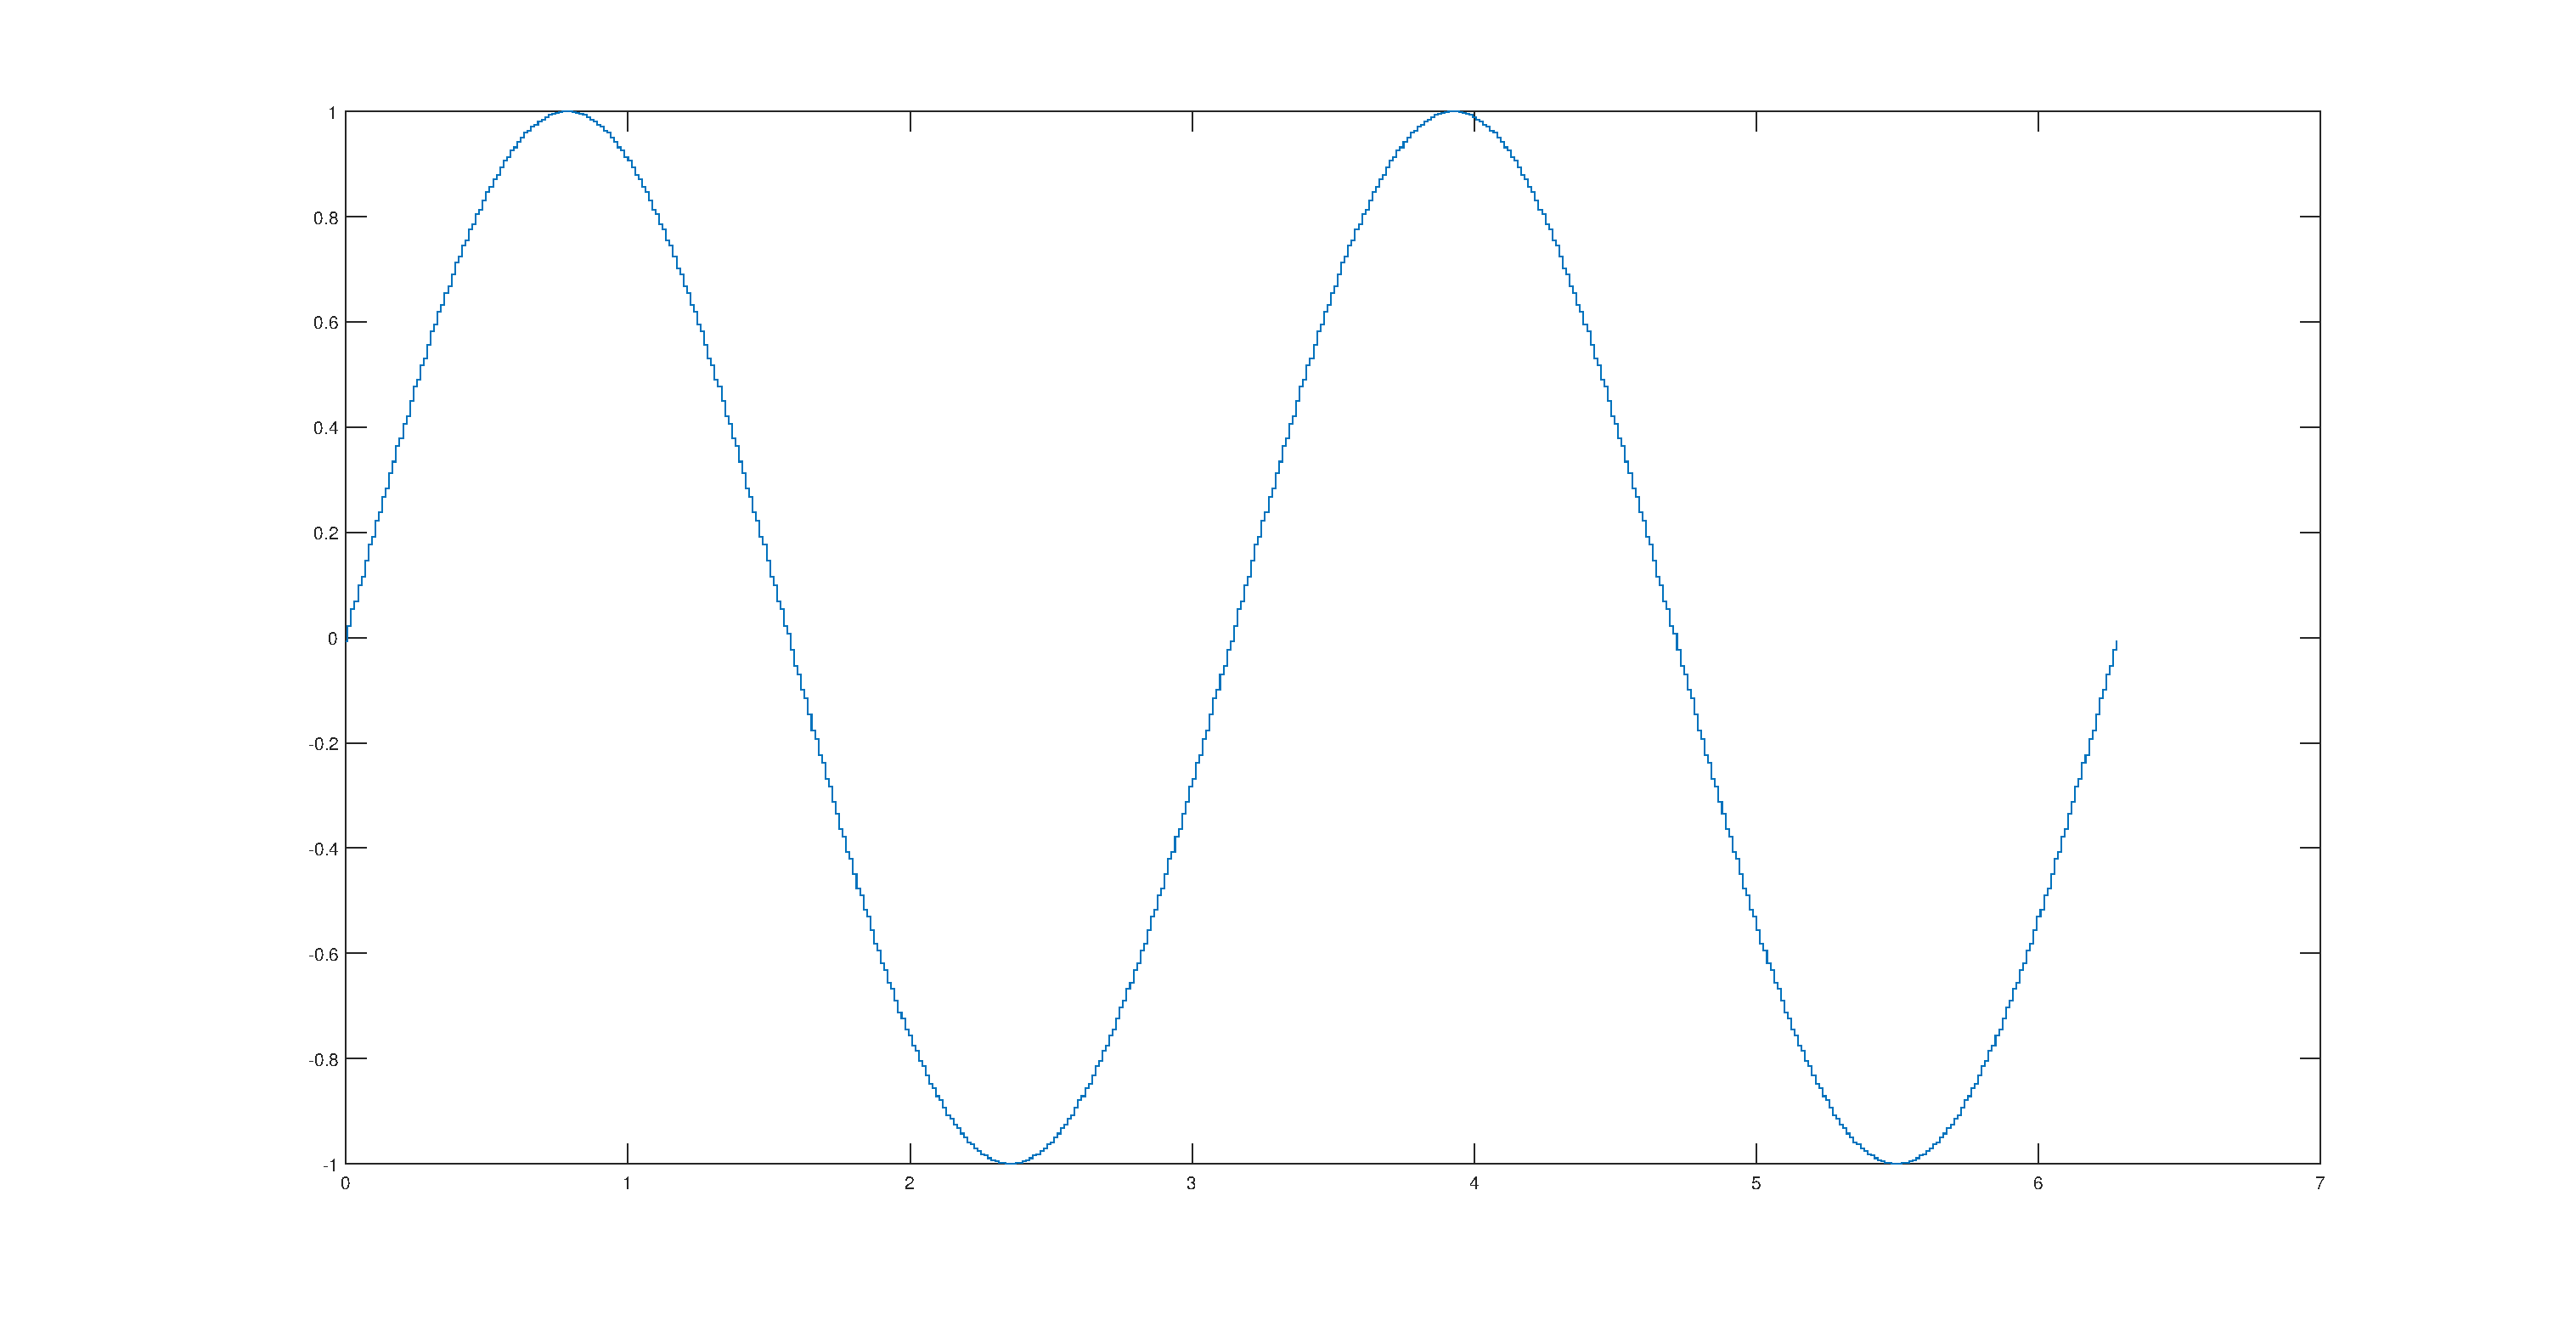
\includegraphics[scale=0.16]{./slike/sin2.eps}
	\caption{\textsl{Sinus duplo veće učestanosti od osnovne}}
	\label{slika:sin2}
\end{figure}

% ------------------ FIR ---------------------------------------------
\subsection{FIR filtar}
U cilju korekcije prenosne funkcije kola zadrške nultog reda projektovan je FIR filtar. Kako bi varijacija amplitude izlaznog signala u opsegu $[\Delta f, f_{max}]$ bila $\pm 0.05$\,dB, potrebno je iznaći najmanji red filtra koji u željenom opsegu dovoljno dobro aproksimira inverznu funkciju funkcije $\sin x/x$. To je obezbeđeno tako što je funkciji \texttt{firls} u \textsl{Python}-u prosleđen niz diskretnih frekvencija i vrednosti željene apmlitude u tim frekvencijama, kao što je na slici \ref{slika:poredjenje} prikazano crvenom bojom.
\vfill
\begin{figure}[h]
	\centering
	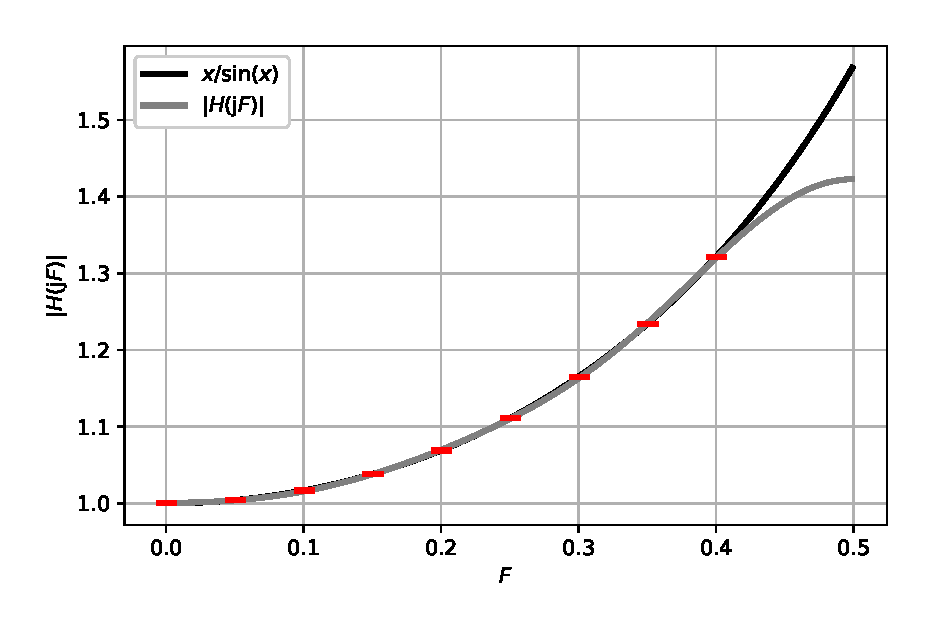
\includegraphics[scale=0.45]{./slike/poredjenje.eps}
	\caption{\textsl{Koeficijenti projektovanog FIR filtra}}
	\label{slika:poredjenje}
\end{figure}
\vfill

Kao rezultat dobijen je FIR filtar osmog reda sa slike \ref{slika:FIR}, čiji su koeficijenti prikazani u tabeli \ref{table:FIR}. \newpage

\begin{figure}[h]
	\centering
	\includegraphics[scale=0.5]{./slike/FIR.eps}
	\caption{\textsl{Koeficijenti projektovanog FIR filtra}}
	\label{slika:FIR}
\end{figure}

\begin{table}[h!]
	\centering
	\caption{Koeficijenti FIR filtra}
	\begin{tabular}{ c|c } 
		Koeficijent		&   Vrednost\\
		\hline
		$h_{invsinc}[0]$ &  $0.00170522$\\ 
		$h_{invsinc}[1]$ &  $-0.00583712$\\ 
		$h_{invsinc}[2]$ &  $0.01786389$\\ 
		$h_{invsinc}[3]$ &  $-0.06833815$\\ 
		$h_{invsinc}[4]$ &  $0.81251125$\\ 
		$h_{invsinc}[5]$ &  $-0.06833815$\\ 
		$h_{invsinc}[6]$ &  $0.01786389$\\
		$h_{invsinc}[7]$ &  $-0.00583712$\\  
		$h_{invsinc}[8]$ &  $0.00170522$\\ 
	\end{tabular}
	\label{table:FIR}
\end{table}


Frekvencijski odzivi kola zadrške nultog reda, projektovanog kompenzacionog FIR filtra i njihov proizvod, prikazani su na slici \ref{slika:nrz_komp}. 

\begin{figure}[h]
	\centering
	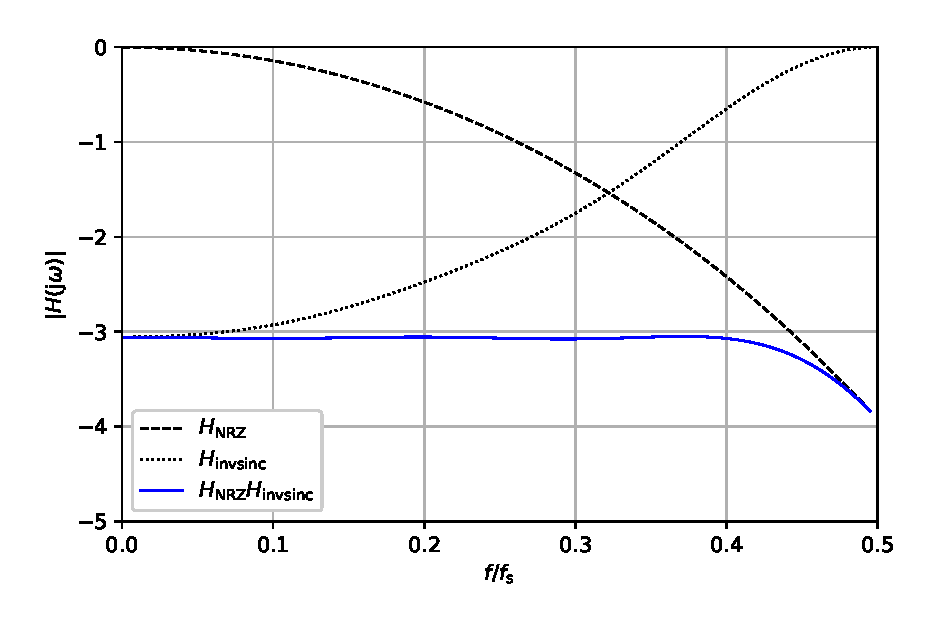
\includegraphics[scale=0.45]{./slike/nrz_komp.eps}
	\caption{\textsl{Kompenzacija NRZ kola}}
	\label{slika:nrz_komp}
\end{figure}

Uvećan prikaz kompenzovanog kola zadrške nultog reda dat je na slici \ref{slika:maxVar}, sa koje se jasno vidi da je amplituda u opsegu $[-3.05, -3.08]$\,[dB], čime su zadovoljeni zahtevani gabariti. \pagebreak

\begin{figure}[h]
	\centering
	\includegraphics[scale=0.5]{./slike/maxVar.eps}
	\caption{\textsl{Varijacija amplitude u opsegu od interesa}}
	\label{slika:maxVar}
\end{figure}

Filtriranje signala je ostvareno pomoću direktne realizacije sa slike \ref{slika:FIRreal}.

\begin{figure}[h]
	\centering
	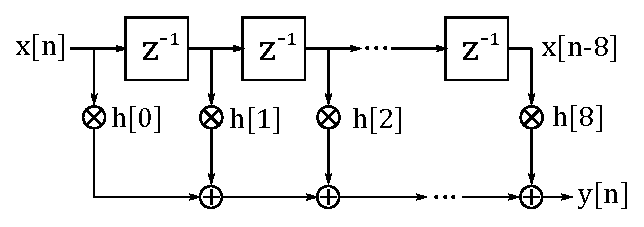
\includegraphics[scale=0.7]{./slike/FIRreal.eps}
	\caption{\textsl{Direktna realizacija FIR filtra}}
	\label{slika:FIRreal}
\end{figure}

% ------------------ Analogni filtar ---------------------------------
\subsection{Analogni rekonstrukcioni filtar}
U cilju suzbijanja spektralnih replika na višim učestanostima, na izlazu DAC-a postavljen je analogni NF filtar. Zbog specifičnog načina preslikavanja spektralnih replika, kao na slici \ref{slika:analogniNF}, moguće je zaći u drugu Nikvistovu zonu za $f_s/2-f_{max}$, tj.~do $f_{stop}=60$\,MHz, čime se dobija prelazna zona NF filtra od $20$\,MHz.
\vfill
\begin{figure}[h]
	\centering
	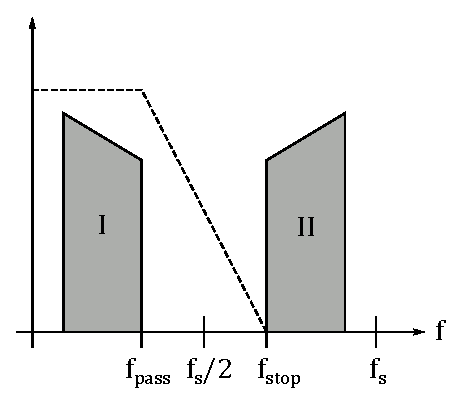
\includegraphics[scale=0.7]{./slike/nikvistAnalog.eps}
	\caption{\textsl{Analogni NF filtar}}
	\label{slika:analogniNF}
\end{figure}
\vfill
Pomoću \textsl{Filter Design \& Analysis Tool}-a u \textsl{Matlab}-u projektovan je Batervortov filtar sa parametrima $F_{pass}=40$\,MHz, $F_{stop}=60$\,MHz, $A_{pass}=0.05$\,dB i $A_{stop}=60$\,dB. Time je dobijen filtar prvog reda, gde je na slici \ref{slika:analogni} prikazan njegov frekvencijski odziv.
\newpage

\begin{figure}[h]
	\centering
	\includegraphics[scale=0.55]{./slike/analogni.png}
	\caption{\textsl{Analogni rekonstrukcioni filtar}}
	\label{slika:analogni}
\end{figure}

% ------------------ Potiskivanje spurova ----------------------------
\subsection{Potiskivanje spurova}
Usled konačne dužine reči za predstavu argumenta generatora odbiraka, dolazi do neuniformne kvantizacije faze. Na slici \ref{slika:kvantFaze} dat je uveličan segment izlaza faznog akumulatora već prikazanog na slici \ref{slika:fazniAcc}.

\begin{figure}[h]
	\centering
	\includegraphics[scale=0.15]{./slike/kvantFaze.eps}
	\caption{\textsl{Neuniformna kvanitzacija faze}}
	\label{slika:kvantFaze}
\end{figure}

 Kao što se d\'a uočiti, razlika između dva uzastopna nivoa nije uniformna, što implicitno uzrokuje neuniformnu kvantizaciju amplitude, usled čega se u spektru izlaznog signala javljaju periodične smetnje, tzv.~spurovi, prikazani na slici \ref{slika:spur}.

\begin{figure}[h]
	\centering
	\includegraphics[scale=0.15]{./slike/spur.eps}
	\caption{\textsl{Spektar izlaznog signala sa uočljivim spurovima}}
	\label{slika:spur}
\end{figure}

Do pojave spurova u spektru dolazi ukoliko je zadovoljena relacija 

\begin{equation}\label{eq:spur}
	\frac{f_{out}}{f_{clk}} = \frac{P}{M} ,
\end{equation}

\noindent gde je $f_{out}$ željena učestanost signala, $f_{clk}$ učestanost odabiranja, $P$ paran broj, a $M=2^m$ broj odbiraka. Jedna od tehnika za razbijanje spurova je tzv.~\textsl{ditering}. Ova tehnika sastoji se od dodavanja nekorelisanog ili pseudoslučajnog signala na ''spurovit`` signal, čime se razbijaju periodične komponente. Na slici \ref{slika:nospur} prikazan je spektar izlaznog signala popravljen nesupstraktivnim diterom, na kom se više ne uočavaju spurovi.

\begin{figure}[h]
	\centering
	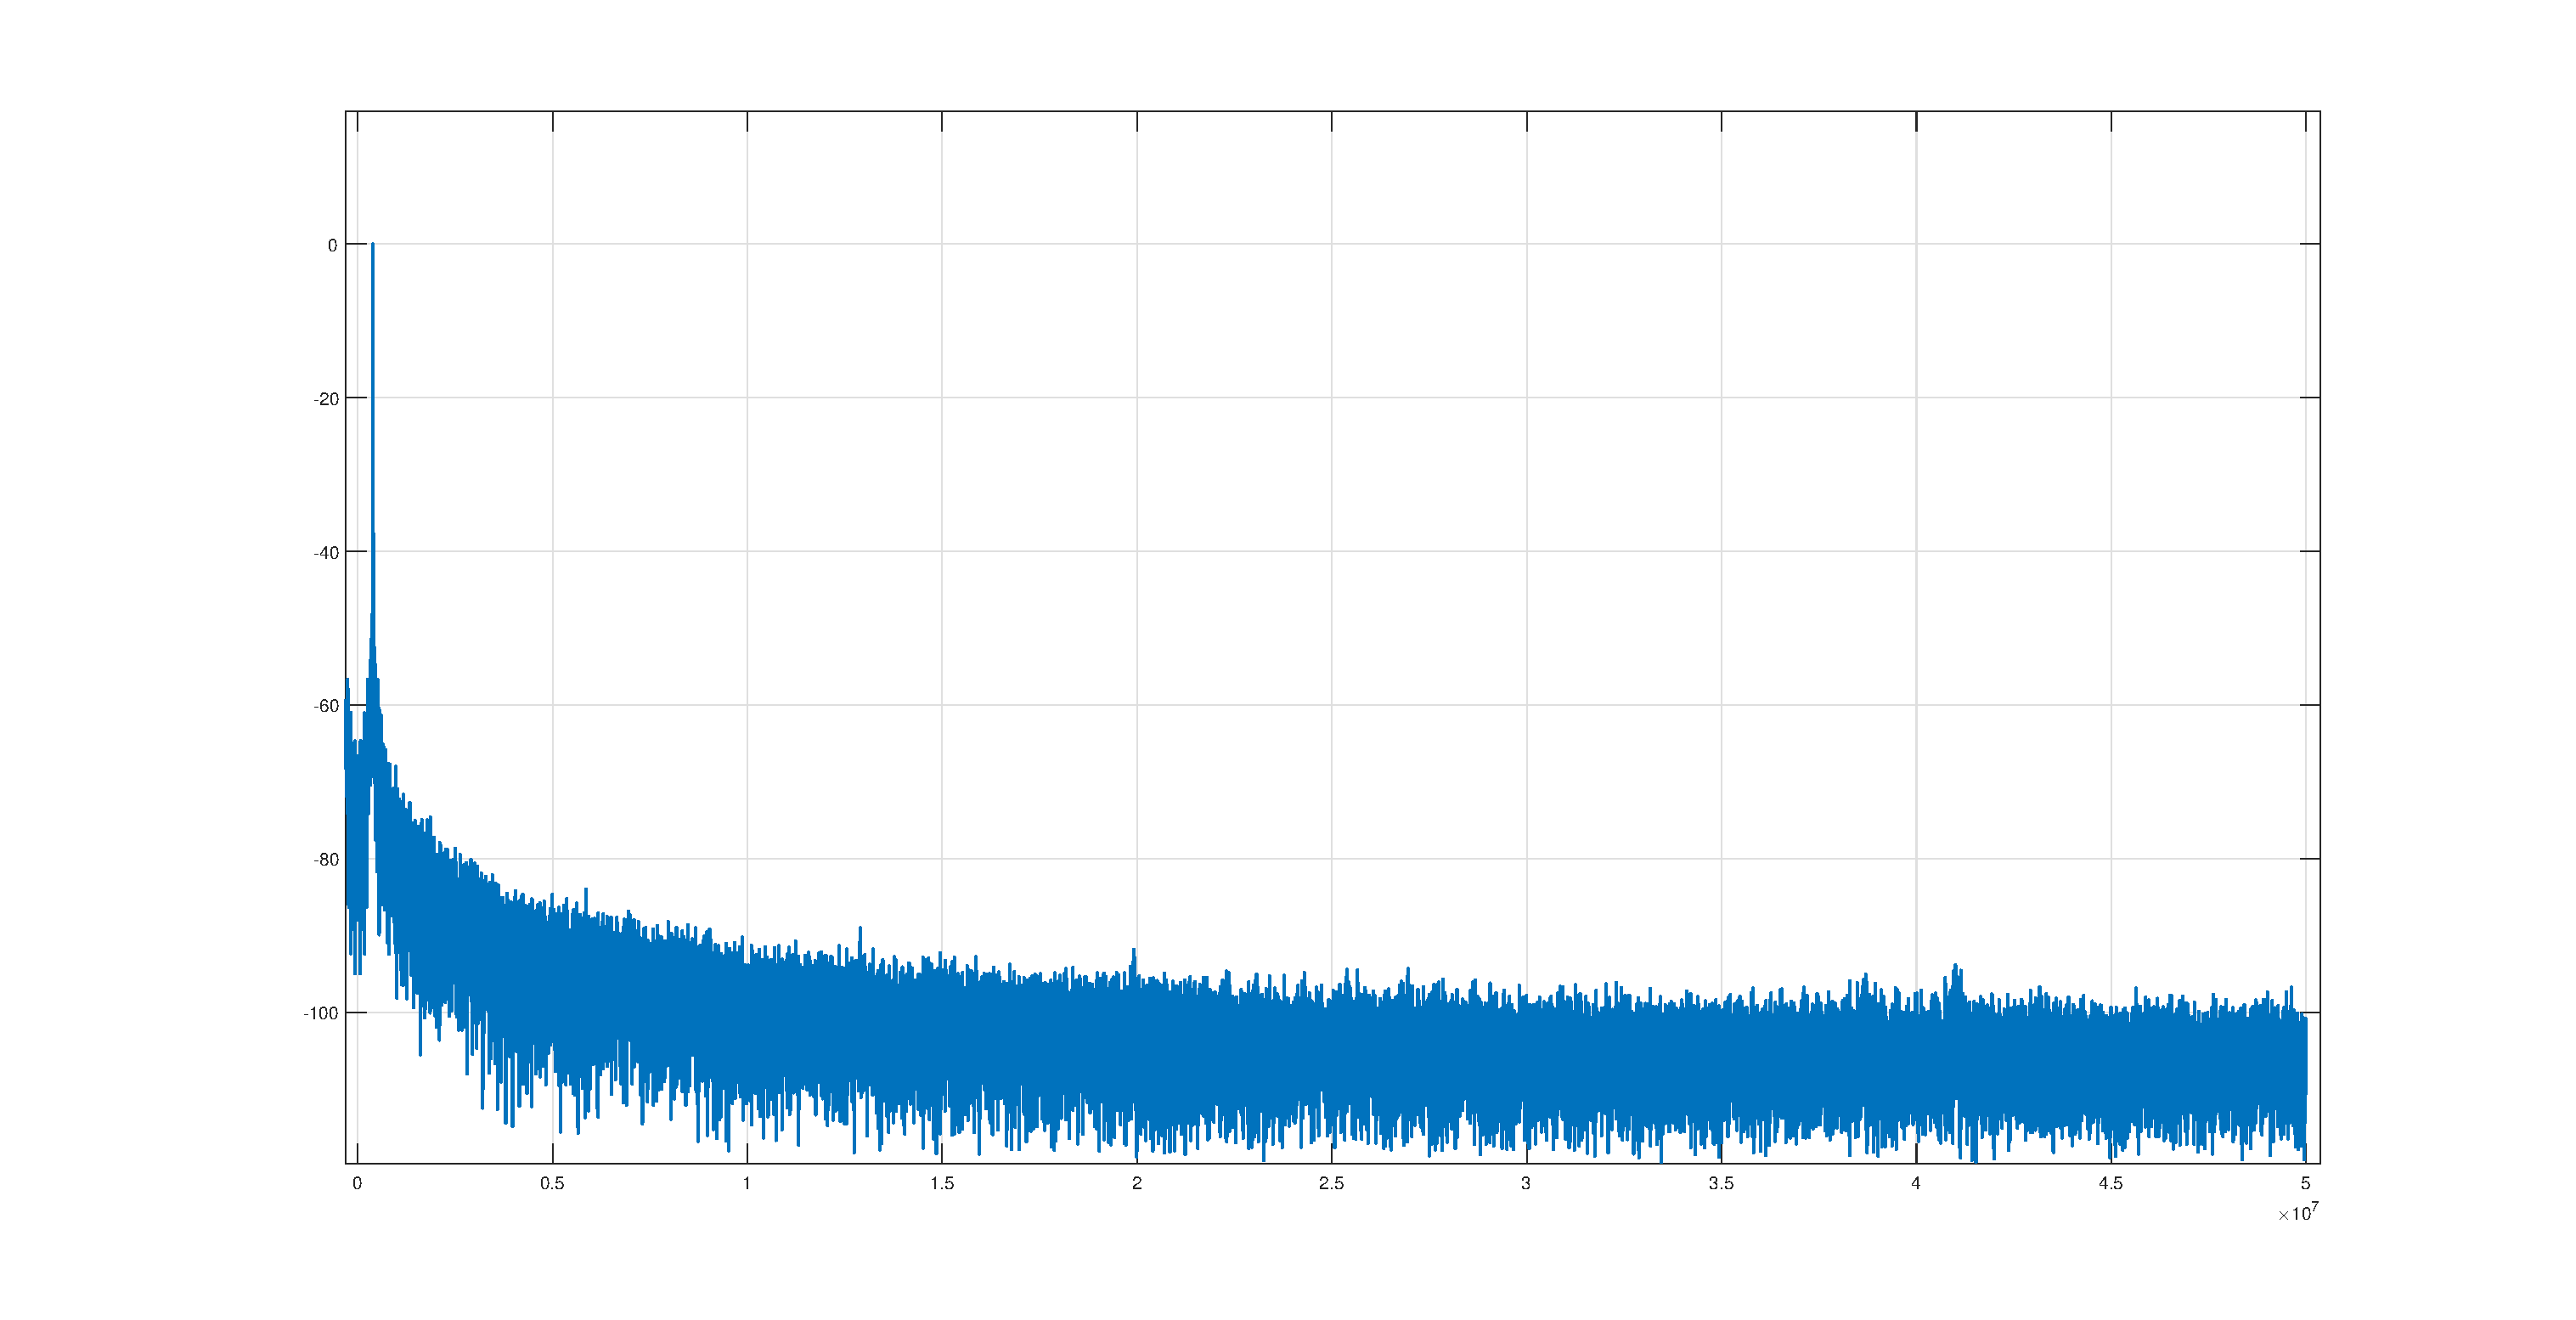
\includegraphics[scale=0.15]{./slike/nospur.eps}
	\caption{\textsl{Spektar izlaznog signala bez spurova}}
	\label{slika:nospur}
\end{figure}

% ------------------ Dziter ------------------------------------------
\subsection{Džiter}
Podrhtavanje takta unosi nesigurnost u trenutke odabiranja signala, čime se efektivno unosi šum u signal. Odnos signal-šum usled džitera takta je 

\begin{equation}
SNR = 10\log_{10}\frac{P_{signal}}{P_{noise}}=20\log_{10}\frac{1}{2\pi f\,t_{j,clk}} .
\end{equation}

Imajući u vidu da je 

\begin{equation}
SNR = SQNR = 6.02N + 1.76\, \text{dB} ,
\end{equation}

\noindent dobija se da je 

\begin{equation}
t_{j,clk} = \frac{1}{2\pi f}\,10^{-\frac{6.02N + 1.76}{20}}  .
\end{equation}

Zamenom $f=f_{max}$ i $N=14$, dobija se $t_{j,clk}\approx 0.2$\,ps. Ovako mali džiter može se realizovati pomoću \textsl{LTC6951} i \textsl{LMX2594} PLL-ova ili \textsl{ADS5401} i \textsl{ADC32RF42} AD konvertora. 

% ------------------ Treca Nikvistova zona ---------------------------
\subsection{Generisanje signala u trećoj Nikvistovoj zoni}
Kolo zadrške nultog reda pogodno je za rekonstrukciju signala u prvoj Nikvistovoj zoni, pošto potiskuje spektralne replike u višim zonama. Rekonstrukcija signala u višim Nikvistovim zonama ostvariva je pogodnim odabirom kola zadrške. Jedan od mogućih izbora je bipolarno kolo zadrške nultog reda kod kojeg slabljenje u trećoj Nikvistovoj zoni ne premašuje $\approx 13$\,dB. Ipak, ovo kolo unosi neravnomerno slabljenje u opsegu $f/fs = [1, 1.5]$, što nije poželjno. Ovaj problem može se prenebregnuti bipolarnim kolom zadrške nultog reda sa povratkom na nulu, sa slabljenjem nešto većim od oko $10$\,dB, ali koje je približno konstantno na pomenutom opsegu.

Takođe, potrebno je modifikovati analogni rekonstrukcioni filtar sa NF na propusnik opsega $[f_s, \frac{3}{2}f_s]$. Kao što se može videti sa slike \ref{slika:nikvist}, ovakav filtar zahtevao bi izuzetno usku prelaznu zonu između $f_s-\Delta f$ koje pripada drugoj i $f_s+\Delta f$ koje pripada trećoj Nikvistovoj zoni. Prelazna zona širine $2\Delta f = 200\,\mu$Hz iziskuje veoma veliki red filtra. Jedino vidno rešenje tog problema je povećanje minimalne učestanosti signala koje bi obezbedilo širu prelaznu zonu i ujedno manji red filtra.

\begin{figure}[h]
	\centering
	\includegraphics[scale=0.7]{./slike/nikvist.eps}
	\caption{\textsl{Replike spektra u višim Nikvistovim zonama}}
	\label{slika:nikvist}
\end{figure}

Najviša Nikvistova zona u kojoj je moguće izvšiti odabiranje je 

\begin{equation}
k_{max} = \floor[\Big]{\frac{f_H}{B}} .
\end{equation}

\noindent Kako bismo obezbedili $k=3$, pri $f_{max}=40$\,MHz, potrebno je da bude $B=12$\,MHz, usled čega se dobija da je

\begin{equation}
\frac{2f_H}{k}\leq f_s\leq \frac{2f_L}{k-1} ,
\end{equation}
\begin{equation}
26.7\,\text{MHz}\leq fs\leq 28\,\text{MHz} .
\end{equation}

Dakle, da bi se obezbedilo odabiranje u trećoj Nikvistovoj zoni sa manjim $f_{clk}$ potrebno je smanjiti širinu prelazne zone na samo $12$\,MHz, čime se zaista obezbeđuje manja učestanost odabiranja, ali opseg učestanosti koji je moguće realizovati postaje značajno manji. Stoga je najbolje zadržati prvobitnu učestanost odabiranja od $f_{clk}=100$\,MHz, a $\Delta f$ povećati dovoljno da se obezbedi šira prelazna zona koja bi omogućila dogledan red prethodno opisanog modifikovanog analognog filtra na izlazu. 
\bigskip 

% ------------------------- Razvojno okruženje ---------------------------------------------------
\section{Razvojno okruženje}\label{sekcija:okruzenje}
Programski kod koji obavlja zahtevanu funkcionalnost sistema napisan je u programskom jeziku \textit{C++}, dok je razvojno okruženje korišćeno za izradu ovog projekta \textit{Visual Studio Code}.

Za potrebe fiksne aritmetike korišćene su biblioteke \texttt{ac\_fixed.h} i \texttt{ac\_int.h}, pri čemu prva omogućava rad sa brojevima sa fiksnim zarezom dok druga biblioteka služi za korišćenje celobrojnih promenljivih ograničenih na određen broj bita.

Funkcionalnost je ostvarena u okviru fajla ''\textit{main.cpp}``. Vrednosti koje se po uslovu zadatka vode na DAC konvertor i određeni međurezultati bivaju smešteni u fajl ''\textit{DDSlog.csv}``, dok fajl ''\textit{logProcess.m}`` predstavlja skriptu koja se pokreće iz \textit{MATLAB}-a i služi za prikaz rezultata smeštenih u okviru \textit{log} fajla.
\bigskip

\section{Funkcionalni blokovi realizovanog sistema}\label{sekcija:kod}
% ------------------------- Fazni akumulator ---------------------------------------------------
\subsection{Fazni akumulator}
Fazni akumulator realizovan je u vidu promenljive \texttt{phaceAcc}. Ova promenljiva, budući da je ograničena širinom od $W=40$ bita, predstavlja broj u opsegu $[0, 2^{40}-1]$. Frekvencija generisanog signala određena je inkrementom faznog akumulatora, označenog sa \texttt{dteta}, pri čemu minimalna vrednost inkrementa predstavlja frekvencijsku rezoluciju. Ipak, budući da su obe promenljive bezdimenzioni brojevi, omogućena je intuitivna manipulacija ovim vrednostima. Imajući u vidu da je najmanji inkrement faznog akumulatora jednak $\Delta \theta_{min}$ = $2^0$ = $1$ i jednačinu (\ref{eq:Minc}) \texttt{dtheta} se računa po formuli
\\
\begin{equation}
\Delta \theta = M_{inc}\,\Delta \theta_{min} = \frac{f_0}{\Delta f} = \frac{f_{0}}{f_{clk}}\,2^W ,
\end{equation}

\noindent pri čemu je sa $f_{0}$ označena učestanost željenog signala a sa $f_{clk}$ učestanost takta. Ovakvim pristupom, korisniku je omogućeno da unese željenu frekvenciju u vidu promenljive \texttt{f0} koja nadalje biva skalirana u odgovarajući inkrement faznog akumulatora, čime u potpunosti biva lišen unošenja neintuitivnih brojeva. Ujedno se za najmanju ostvarivu frekvenciju $\Delta f$ dobija da je $M_{inc}=1$, odnosno, inkrement faznog akumulatora jednak je bitu najmanje težine. Maksimalna ostvariva učestanost ovakvog sistema, $f_s/2$, biva preslikana u inkrementalni pomeraj od $2^{W-1}$, odnosno, u pomeraj koji je jednak $\pi$.

Početna faza, označena sa \texttt{phi}, predstavlja takođe ceo broj dužine $W=40$ bita. Korisnik unosi željenu početnu fazu preko promenljive \texttt{phi0}, pri čemu njena vrednost pripada intervalu $[0, 2\pi]$. Tako unesena vrednost se dalje skalira: kako maksimalni pomeraj od $2^W$ odgovaraja inkrementu faze za $2\pi$, to znači da za $\phi_0 = 2\pi$ inkrement akumulatora mora biti jednak $2^W$. Stoga, početna faza koja se pridodaje faznom akumulatoru računa se po formuli

\begin{equation}
\phi = \frac{\phi_0}{2\pi} 2^W
\end{equation}

Na slici \ref{slika:kos1} prikazan je kosinusoidalni signal čija je učestanost $f_0 = 1$\, MHz. 

\begin{figure}[h]
	\centering
	\includegraphics[scale=0.15]{./slike/kos1.eps}
	\caption{\textsl{Kosinus učestanosti 1\,MHz}}
	\label{slika:kos1}
\end{figure}

Promenom korisnički definisanih parametara na $f_0 = 2$\, MHz i $\phi_0 = \pi/4$ dobija se kosinusoida prikazana na slici \ref{slika:kos2}. Kao što se da videti, učestanost kosinusoide je duplo veća, pri čemu je izvršen fazni pomeraj koji je unet od strane korisnika.

\begin{figure}[h]
	\centering
	\includegraphics[scale=0.15]{./slike/kos2.eps}
	\caption{\textsl{Kosinus učestanosti 2\,MHz i početne faze $\pi$/4}}
	\label{slika:kos2}
\end{figure}

% ------------------ cos x -------------------------------------------
\subsection{Generator odbiraka $cos\,x$}
Izlaz iz faznog akumulatora, promenljiva \texttt{phaseAccOut}, dovodi se na ulaz u \textit{CORDIC} algoritam, gde je nadalje potrebno izračunati vrednost amplitude na osnovu dovedene vrednosti faze.

Kako je maksimalna vrednost ugla koja se može proslediti \textit{CORDIC} algoritmu jednaka $99.88$\textdegree, potrebno je na neki način ograničiti vrednost ugla koja se prosleđuje za izračunavanje amplitude. To je učinjeno tako što se najviših dva bita dovodi na ulaz multipleksera u vidu promeljive \texttt{muxSel}, dok se ostalih $12$ bita koristi za mapiranje vrednosti u opsegu od $[0, \frac{\pi}{2}]$ u vidu \texttt{phaseAccOut}.

Sama \texttt{for} petlja koja realizuje $M=14$ iteracija \textit{CORDIC} algoritma implementira jednačine (\ref{eq:cordicX}) -- (\ref{eq:cordicSigma}). Radi optimizacije, pre samog početka rada napravljena je svojevrsna tabela vrednosti za $\arctan{2^{-i}}$. Budući da se taj niz vrednosti pojavljuje u svakoj iteraciji algoritma, ovim je postignuta manja redudansa kao i brže izvršavanje samog programa. Takođe, imajući u vidu zaključak izveden iz jednačine (\ref{eq:Kinf}), $K(n) = K_{\infty}$ je sračunato pre samih iteracija \textit{CORDIC}-a.

Kod izračunavanja trigonometrijskih funkcija pomoću \textit{CORDIC}-a postavljaju se sledeće početne vrednosti promenljivih: $x_0=K_{\infty}$, $y_0=0$. Ipak, kako kontrolna promenljiva na ulazu u \textit{CORDIC} algoritam, \texttt{phaseAccOut}, a koja bi trebalo da nosi informaciju o željenoj vrednosti ugla $z_0$, nema nikakvu realnu dimenziju, potrebno je izvršiti skaliranje. Budući da je maksimalna vrednost \texttt{phaseAccOut} jednaka $2^{M-2}-1$ i da ona odgovara fazi od $\pi/2$, promenljiva \texttt{z} se računa po formuli:

\begin{equation}
z_0 = \frac{phaseAccOut}{2^{M-2}-1} \frac{\pi}{2} .
\end{equation}

Izlazne vrednosti, $x$ i $y$, smeštaju se zatim u promenljive \texttt{sampleSin} i \texttt{sampleCos}, na osnovu vrednosti promenljive \texttt{muxSel}.


% ------------------------- Diter -----------------------------------------
\subsection{Diter}
Spurovi se javljaju kao neželjene periodične smetnje u spektru izlaznog signala i posledica su neuniformne kvantizacije faze. Pri koherentnom odabiranju uslovljenom jednačinom (\ref{eq:spur}), spurovi su jasno vidljivi u spektru signala, kao što se d\'a videti na slici \ref{slika:spur}.

Taktovanje celog sistema u \textit{C++}-u implementirano je \texttt{for} petljom koja se, na osnovu jednačine (\ref{eq:spur}), izvršava $2^n$ puta, čime je obezbeđeno logovanje celog broja perioda sinusnog signala. U implementaciji je uzeto da je $n=16$, koje omogućava izuzetno brzo izvršavanje programa u \textit{C++}-u, dok, s druge strane, \textit{MATLAB}-u pruža dovoljan broj odbiraka za detaljno iscrtavanje signala i njegovog spektra. Naravno, ovo uzrokuje da je frekvencijski bin u \textit{MATLAB}-u širine $\Delta f=f_{clk}/2^{16}$, a ne $\Delta f=f_{clk}/2^{40}$, ali je dovoljno dobar kompromis između oprečnih zahteva za preciznošću i kratkim vremenom izvršavanja.

Tehnika koja je iskorišćena za razbijanje spurova je tzv.~\textit{ditering}. Ova tehnika sastoji se od dodavanja nekorelisanog ili pseudoslučajnog signala na ''spurovit`` signal, čime se razbijaju periodične komponente. Pseudoslučajan signal u \textit{C++}-u implementiran je instanciranjem objekata \texttt{default\_random\_engine} i \texttt{normal\_distribution} iz \texttt{<random>} biblioteke, koji omogućavaju generisanje slučajnih brojeva sa normalnom raspodelom $\mathcal{N} {\raise.17ex\hbox{$\scriptstyle\mathtt{\sim}$}} (\mu, \sigma^2)$ sa proizvoljnim $\mu$ i $\sigma$. Generisani pseudonasumični brojevi sa $\mu=0$ i $\sigma=1$ pomnoženi su sa $2^{26}$ kako bi se šiftovali do bita koji se prosleđuju \textit{CORDIC} algoritmu, kao i sa \texttt{ditherAmp} čime se podešava nivo ditera koji se dodaje na fazni akumulator u svakoj iteraciji pomenute \texttt{for} petlje.

Na slici \ref{slika:nospur} prikazan je spektar izlaznog signala popravljen nesupstraktivnim diterom, na kom se više ne uočavaju spurovi.

% ------------------------- FIR -----------------------------------------
\subsection{FIR filtar}
FIR filtar za korekciju $\sin x/x$ frekvencijske karakteristike kola zadrške nultog reda implementiran je direktnom realizacijom sa slike \ref{slika:FIRreal}, koja se može matematički zapisati kao

\begin{equation}\label{eq:konv}
y[n] = \sum_{i=0}^{8}{h[i]\,x[n-i]} ,
\end{equation}

\noindent što predstavlja konvoluciju koeficijenata filtra $h[0]\ldots h[8]$ sa trenutnim $x[n]$ i prethodnim $x[n-1]\ldots x[n-8]$ izlazima \textit{CORDIC}-a.

Na identičan način je u nizove \texttt{cordicSin} i \texttt{cordicCos} smeštano poslednjih devet izlaza generatora odbiraka, i ti nizovi su po jednačini (\ref{eq:konv}) konvoluirani sa koeficijentima filtra prethodno izračunatim u \textit{Python}-u tako da filter zadovoljava zahtevane uslove, i smeštenim u \texttt{filter} niz. Rezultati konvolucije, tj.~filtriranja \texttt{DACinputCos} i \texttt{DACinputSin} potom su upisani u izlazni fajl za logovanje.
\bigskip

% ------------------------- Zakljucak -----------------------------------------
\section{Zaključak}
U ovom radu dati su teorijski aspekti nuži za razumevanje rada sistema za direktnu digitalnu sintezu, kao i opis čisto softverske implementacije navedenog sistema u programskom jeziku \textit{C++}. Svi dobijeni rezultati simulacija u potpunosti se slažu sa onim što teorija predviđa.

% ------------------ Reference ---------------------------
\begin{thebibliography}{00}
	\bibitem{b1} Dr.~Dušan Grujić, Predavanja iz predmeta \textsl{Hardversko-softverska obrada signala}, Elektrotehnički fakultet, Beograd\\
	\bibitem{b2} Bruce Land, \textsl{Direct Digital Synthesis}, Cornell University, New York, \\\url{https://www.youtube.com/watch?v=YDC5zaEZGhM}\\
	\bibitem{b3} Analog Devices, \textsl{Fundamentals of Direct Digital Synthesis}, \\\url{https://www.analog.com/media/en/training-seminars/tutorials/MT-085.pdf}\\
	\bibitem{b4} HLS LIBS, \textsl{AC DATATYPES}, \\\url{https://hlslibs.org/#collapseACDatatypes}\\
	\bibitem{b5} C++, \textsl{std::normal\_distribution}, \\\url{http://www.cplusplus.com/reference/random/normal_distribution/}\\
\end{thebibliography}

\end{document}